\documentclass{tufte-handout}
\usepackage{amsmath,amsthm}

\input{vc.tex}  % For version control

\usepackage{booktabs}
\usepackage{graphicx}
\usepackage{tikz}

\newtheorem{claim}{Claim}[section]
\title{Collatz 81}
\date{\GITAuthorDate, rev. \GITAbrHash}
\author{}

\begin{document}
\maketitle




\bigskip\noindent
The $N$th \emph{Collatz sequence} is defined by the following process,
starting with the integer $N$:
\begin{enumerate}
\item if the number is even, divide it by 2,
\item if the number is odd, triple it and add 1.
\end{enumerate}
Continue this process until you reach 1.
\begin{marginfigure}
$c_1$: 1

\noindent $c_2$: 2, 1

\noindent $c_3$: 3, 10, 5, 16, 8, 4, 2, 1

\noindent $c_4$: 4, 2, 1

\noindent $c_5$: 5, 16, 8, 4, 2, 1

\noindent $c_6$: 6, 3, 10,
5, 16, 8, 4, 2, 1.

\noindent $c_7$: 7, 22, 11, 34, 17, 52, 26, 13, 40, 20, 10,
5, 16, 8, 4, 2, 1.

\noindent $c_8$: 8, 4, 2, 1

\noindent $c_9$: 9, 28, 14, 7, 22, 11, 34, 17, 52, 26, 13, 40, 20, 10,
5, 16, 8, 4, 2, 1.

\noindent $c_{10}$:  10,
5, 16, 8, 4, 2, 1.

\end{marginfigure}
\medskip
We will estimate the number of different values in the first million
Collatz sequences, a stream of 132,434,271 values.
To make this interesting, we pretend that we have at our disposal a
Sinclair ZX81 with 1~kB of memory.


\subsection{Algorithm D}

\begin{marginfigure}
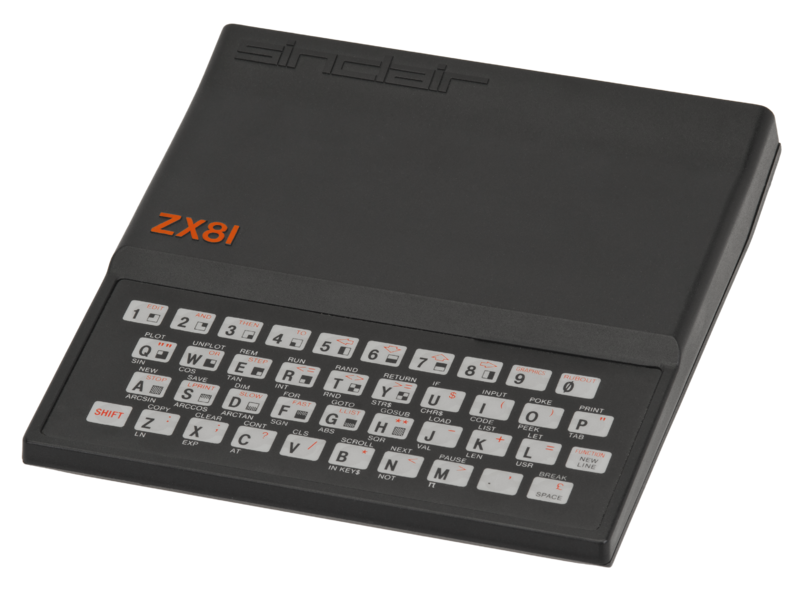
\includegraphics[width=2in]{800px-Sinclair-ZX81.png}
\end{marginfigure}

Algorithm D approximates the number of distinct elements in a stream
of values $x_1,x_2,\ldots$.
We use a pairwise independent hash function $h$ mapping the stream
elements to a range $\{0,\ldots, R-1\}$, where $R$ an integer much
larger than the number of distinct elements we can imagine.
(Typically one will use $R$ to be the number of positive integers
available in a machine word.)
After seeing $i$ elements, the algorithm stores a set $V\subseteq \{
\,(h(x_j),x_j) \mid j=1,\dots,i\,\}$, corresponding to the $t$ distinct
elements having the smallest hash values.
(Ties can be broken arbitrarily.)
When we see the $i$th element $x_i$, we compute its hash value
$h(x_i)$.
If this is smaller than some hash value in $V$, and
$(h(x_i),x_i)\not\in V$, we add $(h(x_i),x_i)$ to $V$ and throw away
an element having the largest hash value.
To estimate the number of distinct elements seen we look at the
largest hash value $v$ in $H$, and compute $tR/v$.
The relative error of this estimate can be shown to be a factor $1\pm
O(t^{-0.5})$ with probability $3/4$.
To increase the confidence to arbitrarily close to 1, run the
algorithm several times (in ``parallel'') and take the median of the
estimates.





\newpage
\section{Collatz 81 Report}


by Alice Cooper and Bob Marley\sidenote{Complete the report by filling
  in your names and the parts marked $[\ldots]$.
  Remove the sidenotes in your final hand-in.}


\subsection{1. Dictionaries}

We let $C_N$ denote the (``flattened'') sequence of the sequences
$c_1,\ldots, c_N$. For instance, $C_3$ is 1, 2, 1, 3, 10, 5, 16, 8, 4,
2, 1.


The following table gives the maximum value appearing in $C_N$, the number
of distinct values in $C_N$ (i.e., the cardinality of $C_N$ viewed as
a set), and the total length of the sequence $|c_1|+\cdots+|c_N|$,
for increasing values of $N$.\sidenote{
    Write a simulator that produces the collatz sequences and computes the
    table values.
    Use a dictionary to compute the  cardinalities, otherwise you'll run
    out of space.}

\medskip
\begin{tabular}{rrrr}
	\toprule
	$N$ & $\max C_N$ & $|C_N|$ & len($C_N$) \\
	\midrule
	10 & 52 & 22 & 77 \\
	100 & 9232 & 251 & 3242 \\
	1,000 & 250504 & 2228 & 60542 \\
	10,000 & 27114424 & 21664 & 859666 \\
	100,000 & 1570824736 & 217212 & 10853840 \\
	1,000,000 & 56991483520 & 2168611 & 132434424 \\
	\bottomrule
\end{tabular}


\subsection{2. Quadratic Time}

The first solution in small space uses the following idea: For given
$N$, produce every value of $C_N$ (without storing the entire
sequence!)
to determine $\max C_N$.
Start a counter at 0.
Then, for every $i=1,\ldots, \max C_N$, produce the entire sequence to
see if $i$ appears.
If so, increase the counter.
The running time will grow as the product of $\operatorname{len}C_N$ and $ \max C_n$.

The largest $N$ for which this idea works within 60 seconds on our
machine was $[\cdots]$.


\subsection{3. Randomized Approximation in Small Space}

The following table shows the output of our implementation of
Algorithm D, together with the error (in percent) relative to the
correct values of $|C_N|$ computed in the first part of the report.

\medskip
\begin{tabular}{rrrr}
  \toprule
  $N$ &   output & relative error \\
  \midrule
  10 & $[\cdots]$ &
  \\
  100 & \\
  1,000 & \\
  10,000 & \\
  100,000 & \\
  1,000,000 & \\
  \bottomrule
\end{tabular}


\newpage
\section{Perspective}

The approximation algorithm is from XXX.

For a nice project idea, install a ZX81 emulator and actually solve
the problem on that, preferably in ZX Basic.
(If you're really cool, get a ZX81.
Or make it run on the hardware of your washing machine or one of those
annoying annoying greeting cards that play \emph{Happy Birthday}.)


\end{document}
